%% Copyright 1998 Pepe Kubon
%%
%% `thes-full.tex' --- the example thesis, FULL version, used
%%                     with  the `csthesis' package 
%% Use: latex thes-full to generate the DVI output, then 
%%      bibtex thes-full to generate the bibliography
%%      makeindex thes-full to get the index, and
%%      latex thes-full (2x) 
%%
%% You are allowed to distribute this file together with all files
%% mentioned in READ.ME.
%%
%% You are not allowed to modify its contents.
%%
\documentclass[11pt]{report}
%\documentclass[11pt,twoside]{report}%% for two-sided printing
\usepackage{pdfpages} 
\usepackage{anysize,fancyhdr,graphics}
\usepackage{csthesis}
\usepackage{makeidx}  %%% standard INDEX
\usepackage[titletoc]{appendix}%%Ensure word appendix appears in toc
\usepackage[pagebackref=true,pdfstartview=FitH,bookmarksopen=false,colorlinks,linkcolor=black,citecolor=black]{hyperref} 

\usepackage{mathrsfs}
\usepackage[noend, algo2e, linesnumbered, ruled]{algorithm2e}
\usepackage{epsfig}
\usepackage{epsf}
\usepackage{graphicx}
\usepackage{subfigure}
\usepackage{graphicx,ctable,booktabs}
\usepackage{hyperref}
\usepackage{multirow}
\usepackage{arydshln}
\usepackage{caption}
\usepackage{amsmath}
\usepackage{afterpage}
\usepackage{amsthm}
\usepackage{mathtools}
\usepackage{amssymb}
\usepackage{epsfig}
\usepackage{color}
\usepackage{algorithm,algorithmic}

\renewcommand{\algorithmicrequire}{\textbf{Input:}}
\renewcommand{\algorithmicensure}{\textbf{Output:}}

\usepackage[export]{adjustbox}

\newtheorem{definition}{Definition}[chapter] 
\newtheorem{property}{Property}[chapter] 
\newtheorem{example}{Example}[chapter] 
%\newtheorem{proof}{proof}[chapter]   
%\newtheorem{lemma}{Lemma}[section]  

%\usepackage{enumitem}
%\setlist{nolistsep}
\renewcommand\arraystretch{1.1}
%\renewcommand{\baselinestretch}{0.96}
\newcommand{\nop}[1]{}

\newcommand{\comment}[1]{{\bf [{\color{blue}\sc from Jian:} {\color{red} #1}]}}
\newcommand{\commentXiaoning}[1]{{\bf [{\color{orange}\sc from Xiaoning:} {\color{blue} #1}]}}

\makeatletter
\def\contentsline#1#2#3#4{%
  \ifx\\#4\\%
    \csname l@#1\endcsname{#2}{#3}%
  \else
    \csname l@#1\endcsname{%
      \hyper@linkstart{link}{#4}{#2}\hyper@linkend
    }{%
      % same link destination for the page:
      \hyper@linkstart{link}{#4}{#3}\hyper@linkend
      % link destination is the page itself:
      % \hyperpage{#3}%
    }%
  \fi
} \makeatother


\makeindex  

%%% The following code demonstrates the ``other list'' facility. A new
%%% command \otherlist is defined for the List of Programs. Programs
%%% are defined as floating environments of type 3 (1 is used for figures,
%%% 2 for tables) and the information about them is stored in an
%%% auxiliary file with .lop extension. You can use this method to
%%% define several types of ``other lists,'' but in that case you'll
%%% need to add appropriate code to \lists in the csthesis.sty
%%% package.
%%% Note: It's better to move this code into your own mythesis.sty
%%% package. If you do that, you should get rid of the \makeatletter,
%%% \makeatother commands.
%\makeatletter
%\newcommand\otherlist{%
%    \addcontentsline{toc}{chapter}{\otherlistname}
%    \if@twocolumn
 %     \@restonecoltrue\onecolumn
%    \else
%      \@restonecolfalse
%    \fi
%    \chapter*{\otherlistname
%      \@mkboth{\MakeUppercase\otherlistname}%
%              {\MakeUppercase\otherlistname}}%
%    \@starttoc{lop}%
%    \if@restonecol\twocolumn\fi
%    }
%\newcommand*\l@program{\@dottedtocline{1}{1.5em}{2.3em}}
%\newcommand\otherlistname{List of Programs}
%\newcommand\programname{Program}
%\newcounter{program}[chapter]
%\renewcommand\theprogram{\thechapter.\@arabic\c@program}
%\def\fps@program{tbp}
%\def\ftype@program{3}
%\def\ext@program{lop}
%\def\fnum@program{\programname~\theprogram}
%\newenvironment{program}
%               {\@float{program}}
%               {\end@float}
%\newenvironment{program*}
%               {\@dblfloat{program}}
%               {\end@dblfloat}
%\makeatother
%%% end of ``other list'' code

\begin{document}
\setlength{\pdfpagewidth}{8.5in}
\setlength{\pdfpageheight}{11in}
%%% set switches
%\contentspagefalse  
\figurespagetrue
\tablespagetrue
\dedicationpagetrue
\quotationpagetrue
%\otherlistpagetrue

%%% front matter 
%% Copyright 1998 Pepe Kubon
%%
%% `titapp.tex' --- title and approval for thes-full.tex, thes-short-tex from
%%                  the `csthesis' bundle
%%
%% You are allowed to distribute this file together with all files
%% mentioned in READ.ME.
%%
%% You are not allowed to modify its contents.
%%

%%%%%%%%%%%%%%%%%%%%%%%%%%%%%%%%%%%%%%%%%%%%%
%
%   Title and approval pages
%
%%%%%%%%%%%%%%%%%%%%%%%%%%%%%%%%%%%%%%%%%%%%%

%%% title page

\title{Individual Skyline Subspace on User Annotated Tags}
\author{Jiaxing Liang}
\qualification{B.Sc., Simon Fraser University, 2013}
\qualification{B.Eng., Zhejiang University, 2013}
\submitdate{Spring 2015}
\copyrightyear{2015}

%%% approval page


\chair{Dr.~Ha Ha,\\
	Associate Professor, } 
\signatory{Dr.~Jian Pei,\\
        Professor, 
%        Computing Science,\\
%       %Simon Fraser University\\ 
       Senior Supervisor}
\signatory{Dr.~Martin Ester,\\
        Professor, 
%        Computing Science,\\
%       %Simon Fraser University\\ 
       Supervisor}
       
\signatory{Dr.~Ha Ha,\\
       Associate Professor,
       %Computing Science,
%       %Simon Fraser University\\ 
       Internal Examiner}


%%% generating title and approval pages 
\beforepreface

 %% title, approval

%% Partial Copyright License (PCL)
%% Please check the library online regulations & Forms, http://www.lib.sfu.ca/thesis
\newpage 			
\addcontentsline{toc}{chapter}{Partial Copyright License}
\mbox{}
\makeatletter
\AddToShipoutPictureBG*{
            \setlength{\@tempdimc}{.06\paperheight}
            \setlength{\unitlength}{1pt}
           \put(\strip@pt\@tempdimb,\strip@pt\@tempdimc){
	\includegraphics{PCL_Declaration.pdf}
	} 
} 
\makeatother
\newpage

% !TEX root = ../topk_thesis.tex
%% Copyright 1998 Pepe Kubon
%%
%% `abstract.tex' --- abstract for thes-full.tex, thes-short-tex from
%%                    the `csthesis' bundle
%%
%% You are allowed to distribute this file together with all files
%% mentioned in READ.ME.
%%
%% You are not allowed to modify its contents.
%%

%%%%%%%%%%%%%%%%%%%%%%%%%%%%%%%%%%%%%%%%%%%%%%%%%
%
%       Abstract    
%
%%%%%%%%%%%%%%%%%%%%%%%%%%%%%%%%%%%%%%%%%%%%%%%%

\prefacesection{Abstract}

Skyline computation is important in applications that involve multi-criteria decision making. In this thesis, we consider the following problem: given a query point, find the subspaces where the query point is in the subspace skyline. Although efficient algorithms for subspace skyline computation were developed in many existing studies, finding skyline subspaces for one certain query point is still an open problem. We develop an algorithm based on bottom-up set enumeration to compute the skyline subspace efficiently. We formulate the problem of identify the uniqueness of a given vertex to skyline subspace queries problem on graph and proposed effective pruning methods to tackle this problem. We further conduct experiments on both real world datasets and synthetic datasets to verify the efficiency of our method.
 %% abstract
%% Copyright 1998 Pepe Kubon
%%
%% `dedquot.tex' --- dedication and quotation for thes-full.tex from
%%                   the `csthesis' bundle
%%
%% You are allowed to distribute this file together with all files
%% mentioned in READ.ME.
%%
%% You are not allowed to modify its contents.
%%

%%%%%%%%%%%%%%%%%%%%%%%%%%%%%%%%%%%%%%%%%%%%%
%
%   Dedication/Quotation pages
%
%%%%%%%%%%%%%%%%%%%%%%%%%%%%%%%%%%%%%%%%%%%%%

\dedication{To my parents.}
\thesquot{%
``You will recognize your own path when you come upon it, because you \\will suddenly have all the energy and imagination you will ever need.''\\[5pt]%
--- \textsc{Jerry Gillies}, (1940- )%
}

%%% generate pages
\dedicquotation
 %% dedication and quotation, if any 
%% Copyright 1998 Pepe Kubon
%%
%% `ack.tex' --- aknowledgments for thes-full.tex, thes-short-tex from
%%               the `csthesis' bundle
%%
%% You are allowed to distribute this file together with all files
%% mentioned in READ.ME.
%%
%% You are not allowed to modify its contents.
%%

%%%%%%%%%%%%%%%%%%%%%%%%%%%%%%%%%%%%%%%%%%%
%
%       Acknowledgment 
%
%%%%%%%%%%%%%%%%%%%%%%%%%%%%%%%%%%%%%%%%%%

\prefacesection{Acknowledgments}
I would like to express my deepest gratitude to my senior supervisor, Dr.~Jian Pei, for his great patience, warm encouragement and continuous support throughout my Master's studies. His wisdom and passion in research has influenced and inspired me a lot, which gave me confidence and interest in accomplishing this thesis. 

I would like to thank Dr.~Martin Ester for being my supervisor and giving me helpful suggestions on my thesis. I also thank Dr.~Ha Ha and Dr.~Ha Ha for serving in my examining committee.  

I am also very grateful to my lab mates for their kind help. A special thank goes to Dr.~Huaizhong Lin, Dr.~Aihua Wu, Dr.~Fuyuan Cao, Dr.~Kui Yu,  Dr.~Dongwan Choi, Guanting Tang, Xiao Meng, Juhua Hu, Chuancong Gao, Yu Yang, Xiangbo Mao, Lumin Zhang, Xiang Wang, Xiaoning Xu, Yu Tao, Lin Liu, Li Xiong, Beier Lu, Zicong Cun, and Xiaojian Wang.

Moreover, my sincerest gratitude goes to my parents for their endless love and support through all these years.






 %%  acknowledgments

%%%  generate contents, lists of figures, etc.
\lists

%% preface (foreword), if any
% \include{files/preface} 

%%% prepare main section
\beforetext

%%% main matter
% !TEX root = ../topk_thesis.tex
%% Copyright 1998 Pepe Kubon
%%
%% `one.tex' --- 1st chapter for thes-full.tex, thes-short-tex from
%%                the `csthesis' bundle
%%
%% You are allowed to distribute this file together with all files
%% mentioned in READ.ME.
%%
%% You are not allowed to modify its contents.
%%

%%%%%%%%%%%%%%%%%%%%%%%%%%%%%%%%%%%%%%%%%%%%%%%%%
%
%       Chapter 1 
%
%%%%%%%%%%%%%%%%%%%%%%%%%%%%%%%%%%%%%%%%%%%%%%%%

\chapter{Introduction}

In this chapter, we first discuss several interesting applications that motivate the problem of continuous similarity search for evolving queries, which will be studied in this thesis.  Then, we will summarize the major contributions and describe the structure of the thesis.

\section{Motivations}

Let us consider a cold-start recommendation problem at a Q\&A website.  Suppose you want to run $3$ advertisements on the Q\&A website for a user who does not have a profile yet, what advertisements should you display?  In addition to many factors, such as click-through rates of advertisements and bidding price information, a natural and important idea is to consider the advertisements  that are most related to the questions being recently asked at the website by all users.  For example, you may want to retrieve the top-$k$ advertisements that are most similar to the last $n$ questions asked, where the similarity measure captures the relevance between advertisements and questions.  Such advertisements can be used as the candidates for further selection. 

The above scenario is just one of the many applications that motivate the problem to be studied in this thesis.  Given a set of static data objects (e.g., ads in the above example), and an evolving data stream (e.g., the questions asked in the above example), a sliding window on the data stream (e.g., the last $n$ questions in the above example) presents an evolving query.  The problem of \emph{continuous similarity search for evolving queries} is to continuously conduct top-$k$ similarity search on the set of static objects using the evolving queries.  

\begin{example}[Motivation Example]\label{motivation}
We are given a set of keywords or phrases for each bidding advertisement as shown in Table~\ref{adskeyword}. At the current moment, assume that the keywords and phrases extracted from the last $10$ questions asked by users in the $Q\&A$ website are $\{$insurance, red cross, A7 chip, fingerprint sensor, Apple, iOS 7, Android, uPass$\}$. Without any further background information, we may assume that a new user may also be interested in some of the topics related to the recent questions asked by all users. Thus, to place advertisements for new users, we simply find the advertisements whose keywords or phrases are, to some extent, similar to those extracted from the recent questions. Suppose we always display the top-$2$ most similar advertisements due to limited space on a webpage and quality user experience, the advertisements displayed for newly-registered users would be $ad_5$ and $ad_2$ based on a predefined similarity measurement, for example, overlap similarity or Jaccard similarity. After a short period of time, say a second, if the keywords and phrases of the most recent $10$ questions have been updated to $\{$fingerprint sensor, Apple, iOS 7, Android, uPass, sneaker, Compass Card, TransLink$\}$. The advertisements recommended for the new users now would be changed to $ad_5$ and $ad_3$.             
\end{example}
 
\begin{table}[t]
     \centering
     \caption{Motivation example: keywords on advertisements}
     %\resizebox{50mm}{!}
     {
\begin{tabular}{|c||p{9cm}|} \hline
      $ad_1$& \{sneaker, outdoor, low-top, Nike, men's\}  \\ \hline
      $ad_2$& \{insurance, donate, treatment, red cross, cord blood\}  \\ \hline
      $ad_3$& \{TransLink, uPass, Compass Card, skytrain\}  \\ \hline
      $ad_4$& \{nikon, lens, megapixels, slr camera\} \\ \hline
      $ad_5$& \{Apple, iPhone 5s, A7 chip, fingerprint sensor\} \\ \hline
      $ad_6$& \{Nexus, tablet, Google, Android, resolution\} \\ \hline
      % Apple, iPad Air, A7 chip, retina, light
\end{tabular}
    }
    \label{adskeyword}
\end{table}

This problem of continuous similarity search for evolving queries has many important applications.  As another example, in a computer war game, a virtual player has a set of weapons and tools, which is relatively stable.  The player goes through a virtual reality space, where the objects in the continuously updated surrounding environment, such as different types of enemies, scoring opportunities, and obstacles, present a stream of evolving queries.  The virtual players has to select proper weapons and tools that match the current surrounding environment best.  Again, before any gaming strategies can be used, an essential task is to continuously maintain the top-$k$ best weapons and tools with respect to the evolving queries.   

% add some other applications
Another interesting application with a similar nature is continuous music recommendation by user humming.  A popular service in Apple app store called \emph{Shazam} can identify a song by taking a short sample of the music. It stores the fingerprints of a comprehensive catalog of music in a database. A song is returned if there is a match in the database regarding the fingerprint of the sample of the song uploaded by the user. However, \emph{Shazam} cannot suggest songs continuously if we play small fractions of several songs in a consecutive way. Thus, we would like to find out a solution to suggest songs continuously using the most recent part of a music stream that consists of small fractions of multiple songs as the query. This application is in demand quite often in daily life. For example, suppose we want to request multiple songs in a KTV song request system and cannot remember the name of each song clearly. Instead of checking the exact song names and searching them in the song request system, it would be much more convenient if the system can suggest the songs continuously when we sing a small part of each song consecutively.    

% Similarly, recognizing handwriting continuously during a user's writing process also motivates our problem.  


% relation between our problem and previous problems

% More generally, a static similarity search problem involves a collection of objects that are characterized by a collection of relevant features, each object being represented as a point in the corresponding attribute space. Given a query as a point in the attribute space, the search is to find the most similar object (also known as nearest neighbour) to the query. 

Our problem can be considered as the dynamic version of the top-$k$ set similarity search problem. More generally, a traditional similarity search problem involves a collection of objects, a similarity function, and a user defined threshold. The search is to find all the objects in the collection whose similarity scores regarding the query are higher than the pre-defined threshold. Similarity search has many applications, such as information retrieval~\cite{SMG83,GG91,FO95}, near-duplicate web page detection~\cite{H06}, record linkage~\cite{W99}, data compression~\cite{GG91}, data integration~\cite{C98}, image and video search and recommendation~\cite{FBFNPE94,FSNAHDGHLPSY95,PPS94,SJ97}, statistics and data analysis~\cite{DW82,KK95}, machine learning~\cite{CS93}, and data mining~\cite{HT95,BMS07}. Besides answering threshold-based queries, top-$k$ queries are also of great value since given a threshold, the size of the result may be unpredictable and, in many real applications, we are only interested in a small number of most similar objects. Moreover, as to be reviewed in Section~\ref{sec:cont-topk}, the problem of similarity search on data streams has been extensively explored, especially for nearest neighbour search.  However, to the best of our knowledge, the problem of continuous similarity search for evolving queries has not been systematically investigated. 

\section{Contributions}
In this thesis, we tackle the problem of continuous similarity search for evolving queries. Since in many applications, an object can be represented as a multi-set, such as using a keyword vector to represent a document, we consider static objects as multi-sets, and use weighted Jaccard similarity as the measure.  The major challenge is how to speed up the similarity computation and avoid checking evolving queries with every static object exactly at every time point. We make the following contributions.  

\begin{itemize}
\item We formulate the problem of \emph{continuous similarity search for evolving queries} that continuously finds the top-$k$ objects in a collection of sets that are most similar to an evolving query.
\item We develop upper bounds for incremental maintenance of similarity scores.  Those bounds can be computed in constant time.
\item We propose algorithms based on two general frameworks.  The first one is \emph{pruning and verification}.  The other one is \emph{hashing}. The pruning-based method reduces the cost of computing the exact similarity scores using pruning strategies. The MinHash-based method estimates Jaccard similarity scores based on MinHash technique~\cite{Broder97} and uses indexing structures for efficient updates.
\item We report an empirical evaluation on both synthetic and real-world data sets, which validates the efficiency and effectiveness of our proposed methods.
\end{itemize}
  

\section{Organization of the Thesis}
The rest of the thesis is organized as follows. In Chapter~\ref{ch:related-work}, we review the related work. We then formulate the problem of \emph{continuous similarity search for evolving queries} in Chapter~\ref{ch:prob-def}. In Chapter~\ref{ch:pruning}, we propose a pruning-based method.  In Chapter~\ref{ch:hashing}, we present a MinHash-based method.  We report our experimental results in Chapter~\ref{ch:exp}, and conclude the thesis in Chapter~\ref{ch:con}.










 
%% Copyright 1998 Pepe Kubon
%%
%% `two.tex' --- 2nd chapter for thes-full.tex, thes-short-tex from
%%               the `csthesis' bundle
%%
%% You are allowed to distribute this file together with all files
%% mentioned in READ.ME.
%%Discuss the reality where queries are not randomly generated.
%% You are not allowed to modify its contents.
%%

%%%%%%%%%%%%%%%%%%%%%%%%%%%%%%%%%%%%%%%%%%%%%%%%%
%
%     Chapter 2   
%
%%%%%%%%%%%%%%%%%%%%%%%%%%%%%%%%%%%%%%%%%%%%%%%%

\chapter{Related Work}
\label{ch:related-work}

Our problem of \emph{skyline subspace query} is mainly related to the existing work on general skyline query, subspace skyline computation and skyline query with specific constrain which are reviewed in Section~\ref{sec:rel:general}, Section~\ref{sec:cont-topk} and Section~\ref{sec:rel:constrain}, respectively.

\section{General Skyline Query}
\label{sec:rel:general}

A number of studies of skyline done before. Borzsony et al~\cite{borzsony2001skyline} proposed the Block Nested Loop (BNL) method to compute the general skyline queries. Their work was more about finding the skyline points efficiently in Database.

\section{Subspace skyline computation}
\label{sec:rel:subspace}

For subspace skyline problem, Pei et al~\cite{pei2005catching}proposed the \emph{Skyey} algorithm which is based on the property of decisive subspaces to compute the skyline points for every subspace and the skyline groups and their signatures. Yuan et al~\cite{yuan2005efficient} developed the \emph{Top-Down Skyline Algorithm} to compute the skyline in every subspace. They also developed a novel data structure \emph{skylist} to store skyline
objects in different subspaces in a compact way. In our paper, we are focusing on one query point not the whole dataset. Our work is to find the subspaces in terms the query point. We also extend our work on the graph setting and spatial setting.

\section{Skyline Query with Specific Constrain}
\label{sec:rel:constrain}
% add data stream models
In this section, we briefly review various data stream models. Since our problem shares many common characteristics with continuous query answering over a data stream, we then review related problems including but not limited to similarity search.  

\subsection{Data Stream Models}
A data stream is a sequence of data elements $a_1, a_2, \dots$ that arrives item by item, which describes an underlying signal. The signal is a one-dimensional function $A: [1...N] \mapsto R$, where the domain consists of integers and the range is the set of real numbers. As mentioned in~\cite{muthukrishnan05}, there are mainly three models that differ on how items describe the signal, namely, time series model, turnstile model, and cash register model. We summarize the models briefly as the following.  

\begin{itemize}
\item \textbf{Time Series Model} This is the simplest model in which each $a_i$ is equal to $A[i]$ and items show up in the increasing order of $i$. We can think of the daily closing price of a stock from the listing date to the present as a data stream. Each $a_i$ corresponds to the closing price of the stock at day $i$.          

\item \textbf{Turnstile Model} In this most general model, $a_i = (j, U_i)$ which is an update to $A[j]$ where $U_i$ can be any real number. Suppose $A_i$ is the signal after processing the $i^{th}$ item $a_i$ in the stream, the update can be written as $A_i[j] = A_{i-1}[j] + U_i$. Let us consider a scenario where $N$ investors buy and sell shares of a certain stock. Since investors can buy and sell stock without particular order, a data stream, i.e., a sequence of transactions, $a_1, a_2, \dots$, can be generated. The $i^{th}$ transaction $a_i = (j, U_i)$ indicates that investor $j$ wants to buy $|U_i|$ shares if $U_i > 0$ and sell $|U_i|$ shares otherwise. Then, the total shares held by investor $j$ is updated by $A_i[j] = A_{i-1}[j] + U_i$.       

\item \textbf{Cash Register Model} It can be considered as a special case of the Turnstile model where $U_i \geq 0$. To be more specific, each $a_i=(j, U_i)$ is an increment instead of a general update to $A[j]$. Following the previous example, if investors can only buy shares of stocks, the transaction sequence fits the cash register model. 

\end{itemize}

Many streaming algorithms are designed for the entire data stream. However, a wide range of real applications, such as web log mining and stock market prediction, do not consider outdated elements important. Thus, the sliding window model is of great importance. In this model, we only consider the most recent part of the data stream. Typically, there are two types of sliding windows with equal importance. The count-based sliding window is of fixed size and contains the last $n$ items in the data stream. The time-based sliding window allows bursts at a single time unit since it contains the items that arrived in the last $n$ time units. In this thesis, we focus on the count-based sliding window.   

\subsection{Answering Continuous Queries}

Different evolving models are used in previous studies that investigated continuous queries over a data stream. For example, Kontaki~\textit{et~al.}~\cite{KP04} studied similarity range queries in streaming time sequences using Euclidean distance, where both the query and data objects are evolving. An indexing method that is based on incremental computation method for Discrete Fourier Transform is used for achieving high candidates ratio. Lian~\textit{et~al.}~\cite{DBLP:conf/dasfaa/LianCW07} tackled the similarity search problem over multiple stream time series, given a static time series as a query. An approximation algorithm is developed using a weighted locality sensitive hashing technique. 

Motivated by a wide range of applications such as network intrusion detection, much work~\cite{DBLP:conf/icde/BohmOPY07, DBLP:conf/vldb/KoudasOT004, DBLP:journals/tkde/MouratidisP07, DBLP:journals/tkde/MouratidisPBT05} has been embarked on monitoring nearest neighbour (NN) queries continuously over a data stream. The basic idea is to utilize indexing structures for reducing memory consumption and supporting efficient updates. Mouratidis~\textit{et~al.}~\cite{DBLP:journals/tkde/MouratidisP07} proposed two approaches for continuous monitoring of NN queries over sliding window streams.  The first approach extends the conceptual partitioning method to the sliding window model. Skyline maintenance techniques and pre-computation of future changes in nearest neighbours are used in the second approach.  Koudas~\textit{et~al.}~\cite{DBLP:conf/vldb/KoudasOT004} developed an approximation algorithm that utilizes an indexing scheme, DISC, and has guaranteed error and performance bound.

The existing work on continuously monitoring nearest neighbours for mobile query object is different from the problem studied here. In those previous studies, the mobile object is assumed to move in a trajectory, potentially predictable to some extent.  In this thesis, the stream presenting an evolving query is not assumed a moving object.  Instead, we simply use the current sliding window as the current query.  The existing methods on continuous nearest neighbour monitoring for mobile objects cannot solve our problem.

% To continuously querying the top-$k$ correlated graphs in a data stream scenario, Pan and Zhu~\cite{PZ12} proposed a two-level candidate checking scheme, one corresponding to the potential global candidate, and the other corresponding to the local candidate. This method can discover the emerging candidate patterns without processing the historical global data repetitively. 
Besides continuous queries on similarity search problems, some interesting work is done for graph streams and general functions defined over data streams. Pan and Zhu~\cite{PZ12} developed a two-level candidate checking scheme for continuously querying the top-$k$ correlated graphs in a data stream scenario where static queries are posed on evolving graph streams. Mouratidis~\textit{et~al.}~\cite{DBLP:conf/sigmod/MouratidisBP06} proposed two approaches for continuously answering top-$k$ queries where the query is a static preference function over a fixed-sized sliding window. One approach is to compute new answers whenever a current top-$k$ point expired and the other approach is to precompute future changes partially. 

Our proposed methods aim at providing algorithmic frameworks on how to deal with similarity search over evolving queries.  In our problem, we can take advantage of the fact that consecutive queries in a stream are very similar.  This results in some important design in our algorithms, which distinguishes our methods from the previous ones.  For example, we derive an upper bound on similarity scores after a few updates based on how the queries evolve.  The pruning-based algorithm uses this bound to prune unpromising candidates.  In the hashing-based algorithm, we maintain fixed-length signatures for all transactions and a query.  Since consecutive queries share a large portion of items, the change in the signature of the query is small.  With the help of inverted index, we can further speed up the updates of similarity scores.      

% Yu~\textit{et~al.}~\cite{DBLP:conf/icde/YuPK05} developed two grid-based methods that indexes data objects or query objects for answering $k$-NN queries over moving objects.  

% Kontaki~\textit{et~al.}~\cite{KPM12} considered the problem of answering continuous top-$k$ dominating queries that ranks multidimensional points regarding their dominance power based on a sliding window. Their methods are based on event scheduling techniques, which aim for reducing costly computations. 

% The general idea is to reduce computation cost utilizing the fact that queries are evolving. Thus, we can think of how the evolvement of the query may affect the query results. 

 







%% Copyright 1998 Pepe Kubon
%%
%% `two.tex' --- 2nd chapter for thes-full.tex, thes-short-tex from
%%               the `csthesis' bundle
%%
%% You are allowed to distribute this file together with all files
%% mentioned in READ.ME.
%%
%% You are not allowed to modify its contents.
%%

%%%%%%%%%%%%%%%%%%%%%%%%%%%%%%%%%%%%%%%%%%%%%%%%%
%
%     Chapter 3   
%
%%%%%%%%%%%%%%%%%%%%%%%%%%%%%%%%%%%%%%%%%%%%%%%%

\chapter{Problem Definition}
\label{ch:prob-def}

The traditional skyline query problem is to find the skyline points which are not dominated by any other points. In this thesis, we consider a variant of this problem. We consider a set of objects $S$ in an $n$-dimensional space and a query object $u$ in this space. The object $u$ may be a skyline point in some subspaces. We call these subspaces \emph{skyline subspaces}. The skyline subspaces query is to find out the \emph{skyline subspaces}. Different from the work of Tao et al.~\cite{tao2006subsky}: given a \emph{subspace} as a query, determine the sets skyline points in that subspace, the problem we want to solve is in a reverse way: given a query \emph{point}, determine the subspaces where the query point is in the subspace skyline. In this chapter, we will introduce the general skyline subspace queries and its applications in two different settings: skyline queries on graph and spatial skyline queries.

\section{General Skyline Subspace Queries}

\begin{definition}[Skyline]
For objects $u, v \in S$, $u$ dominates $v$ if and only if for all i, $(1 \leq i \leq n)$, $u.D_i \leq v.D_i$ and there exists a $j$ ($1 \leq j \leq n$) such that $u.D_j < v.D_j$. Object $u$ is a \emph{skyline object} if $u$ is not dominated by any other objects in $S$.
\end{definition}

\begin{definition}[Skyline Subspace]
Subspace $\mathcal{B}$ is a (non-trivial) $|\mathcal{B}|$-dimensional subspace of $\mathcal{D}$ 
if $\mathcal{B}\subseteq \mathcal{D} (\mathcal{B}\neq\emptyset)$.
For an object $u$ in space $\mathcal{D}$, 
the \emph{projection} of $u$ in subspace $\mathcal{B}$, denoted by $u_\mathcal{B}$
, is a $|\mathcal{B}|$-tuple$(u.D_{i_1},\dots,u.D_{i_{|\mathcal{B}|}})$,
where $D_{i_1},\dots,D_{i_{|\mathcal{B}|}} \in \mathcal{B}$, $u.D_i$ is the value of $u$ on $D_i$. If $u_\mathcal{B}$ is not dominated by any $w_\mathcal{B}$ in subspace $\mathcal{B}$ where $w \in S$, then $\mathcal{B}$ is a \emph{skyline subspace} for $u_\mathcal{B}$.
\end{definition}

\begin{definition}[Minimal Skyline Subspace]
A \emph{skyline subspace} $\mathcal{B}$ is a \emph{minimal skyline subspace} for object $u$ if and only if there is no such a \emph{skyline subspace} $\mathcal{C}$ for object $u$ that $\mathcal{C} \subset \mathcal{B}$.
\end{definition}

\begin{definition}[Skyline Subspace Queries]
Given a set of objects $S$ in an $n$-dimensional space $\mathcal{D} = (D_1,\dots,D_n)$ and a query object $u = (u.D_1,\dots,u.D_n)$ in space $\mathcal{D} = (D_1,\dots,D_n)$. The skyline subspaces query is to find all the \emph{minimal skyline subspaces} for query object $u$.
\end{definition}

\begin{table}[h]
    \centering
    \begin{tabular}{|l|l|l|l|}
    \hline
    points & $A$ & $B$ & $C$ \\ \hline
    $x$      & 4 & 2 & 3 \\ \hline
    $y$      & 3 & 3 & 3 \\ \hline
    $z$      & 2 & 4 & 1 \\ \hline
    \end{tabular}
    \caption{\label{tab:objects_example} A set of objects as our running example}
\end{table}

In Table~\ref{tab:objects_example}, if the query point is $y$, the minimal skyline subspaces of $y$ are $(A, B)$ and $(B, C)$. In subspace $(A, B)$, $x_{(A, B)} = (4, 2), y_{(A, B)} = (3, 3), z_{(A, B)} = (2, 4)$ and $y_{(A, B)}$ is not dominated by $x_{(A, B)}$ or $z_{(A, B)}$. 
In subspace $(B, C)$, $x_{(B, C)} = (2, 3), y_{(B, C)} = (3, 3), z_{(B, C)} = (4, 1)$ and $y_{(B, C)}$ is not dominated by $x_{(B, C)}$ or $z_{(B, C)}$. Therefore, $(A, B)$ and $(B, C)$ are both skyline subspaces. 
In subspace $(A, C)$, $y_{(A, C)} = (3, 3), z_{(A, C)} = (2, 1)$ and $y_{(A, C)}$ is dominated by $z_{(A, C)}$. There $(A, C)$ is not a skyline subspace. 
$(A, B, C)$ is a skyline subspace but it not a minimal skyline subspace because it is a proper superset of one of the skyline subspace $(A, B)$.

\section{Skyline Subspace Queries On Graph}
In this section, we introduce the skyline subspace queries on the graph setting. First, we will introduce a kind of graph such that each vertex in the graph contains several labels, denoted by a \emph{label graph}. We are interested in the distance between each vertex and each label. The set of distances between a vertex and all labels is represented by the \emph{label distance vector} of that vertex. The following shows the definitions of \emph{label graph} and \emph{label distance vector}.

\begin{definition}[Label Graph]
A label graph is defined as a undirected and unweighted graph $G = (V, E, L)$, with each vertex $v \in V$ contains a set of labels $L_v \subseteq \mathcal{L}$. $\mathcal{L}$ is the universal set of labels.
\end{definition}

\begin{definition}[Label Distance Vector On Graph in $H$-hop]
Given a label graph $G$ and a hop number $D$, Label Distance Vector of a vertex $v$ is $LV_v=\left\{\left(l_i, dist_i\right)\right\}$, $i = 1 \ldots n$. $l_i$ is a reachable label from $v$. $dist_i$ is the distance from vertex $v$ to the closest vertex that contains label $l_i$. If a label $l_j$ is not reachable by a vertex $u$ in $H$ hops, then $dist_j = \infty$
\end{definition}

\begin{definition}[Skyline Subspace Queries On Graph]
Given a label graph $G = (V, E, L)$, a query vertex $q$ and a number $H$, the skyline subspaces query on graph is to find all the \emph{minimal skyline subspaces} of $q$ in terms of the label distance vectors on graph.
\end{definition}

\begin{table}[h]
    \centering
    \begin{tabular}{|l|l|}
    \hline
    Skills         & Experts \\ \hline
    Accounting     & $u$     \\ \hline
    Bioinformatics & $y, w$  \\ \hline
    C++            & $w$     \\ \hline
    \end{tabular}
    \caption{\label{tab:skill_sets}An example of skill sets on LinkedIn profile}
\end{table}
    
\begin{figure}[h]
    \centering
    \includegraphics[width=0.3\textwidth]{figs/graph_example}
    \caption{\label{fig:graph}An example of LinkedIn network}
    
\end{figure}

Consider an example on LinkedIn to illustrate the skyline subspace queries on graph. In Figure~\ref{fig:graph}, a graph is represented by the LinkedIn connection network. Table~\ref{tab:skill_sets} shows the skills of each person of the LinkedIn network which can be treated as vertices with labels. 
Both of them together represent a \emph{label graph}. In Table~\ref{tab:skill_sets}, it shows that vertex $u$ has a skill of Accounting, vertex $w$ has skills of Bioinformatics and C++ and vertex $y$ has a skill of Bioinformatics. In this example, we want to compute the subspace skyline queries in $3$ hops.

\begin{table}[h]
    \centering
    \begin{tabular}{llll}
    \hline
        Distances & A & B & C \\ \hline
        $u$       & 0 & 2 & 3 \\ \hline
        $v$       & 1 & 3 & $\infty$ \\ \hline
        $w$       & 3 & 0 & 0 \\ \hline
        $x$       & 2 & 2 & 3 \\ \hline
        $y$       & 2 & 0 & 1 \\ \hline
        $z$       & 1 & 1 & 2 \\ \hline
    \end{tabular}
    \caption{\label{tab:distances_graph} distances between each person and each skill}
    
\end{table}

In the header row of Table~\ref{tab:distances_graph}, $A$, $B$ and $C$ stand for Accounting, Bioforinformatics and C++ respectively. The table shows the distances between each person and each skill. For example, the distance between $v$ and skill $B$ is $3$ because $y$ is the closest vertex to $v$ that contains label $B$ and the distance between $v$ and $y$ is $3$. Since C++ is not reachable by $v$ in $3$ hops, the distance between $v$ and $C$ is $\infty$. Each row of Table~\ref{tab:distances_graph} represents a \emph{label vector} of a vertex.
In this example, if the query point is $z$, the minimal skyline subspaces of $z$ are $(A, B)$ and $(A, C)$ because there is no such a vertex $w \in S$ that $w_{(A,B)}$ dominates $z_{(A,B)}$ or $w_{(A,C)}$ dominates $z_{(A,C)}$.


\section{Spatial Skyline Subspace Queries}

In this section, we will introduce spatial skyline subspace queries. Given a set of points in $2$-dimensional space. Some of the points will contain some labels. The distance between a point and a label is the Euclidean distance between that point and the closest point containing that label. Our goal is to compute the skyline subspace queries on this spatial setting.

\begin{definition}[Spatial Label Distance Vector]
Given a set of points $P$, the Label Distance Vector of a point $v$ is $LV_v=\left\{\left(l_i, dist_i\right)\right\}$, $i = 1 \ldots n$. $l_i$ is a reachable label from $v$. $dist_i$ is the Euclidean distance from vertex $v$ to the closest vertex that contains label $l_i$.
\end{definition}

\begin{definition}[Spatial Skyline Subspace Queries]
Given a set of points $P$ and a query point $q$, the skyline subspaces query on Euclidean space is to find all the \emph{minimal skyline subspaces} in terms of the spatial label distance vectors.
\end{definition}

\begin{table}[h]
    \centering
    \begin{tabular}{|l|l|}
    \hline
    Categories     & Spots \\ \hline
    Asian Food     & $u$     \\ \hline
    Breakfast      & $y, w$  \\ \hline
    Cafes          & $w$     \\ \hline
    \end{tabular}
    \caption{\label{tab:spot_category} an example of spots with categories}
    
\end{table}


\begin{figure}[h]
    \centering
    \includegraphics[width=0.5\textwidth]{figs/spatial_figure}
    \caption{\label{fig:spatial_map}An example of spatial locations of spots}
    
\end{figure}

Table~\ref{tab:spot_category} shows different spots with different categories. Figure~\ref{fig:spatial_map} shows the geometric locations of all spots. We consider each spot as a point in a $2$-dimensional space and the categories the spot contains as its labels.

\begin{table}[h]
    \centering
    \begin{tabular}{llll}
    \hline
    Distances & A & B & C \\ \hline
    $u$       & 0 & $\sqrt{5}$ & $\sqrt{10}$ \\ \hline
    $v$       & $\sqrt{2}$ & $\sqrt{13}$ & $\sqrt{18}$ \\ \hline
    $w$       & $\sqrt{10}$ & 0 & 0 \\ \hline
    $x$       & $\sqrt{5}$ & $\sqrt{2}$ & $\sqrt{5}$ \\ \hline
    $y$       & $\sqrt{5}$ & 0 & 1 \\ \hline
    $z$       & $\sqrt{2}$ & 1 & 2 \\ \hline
    \end{tabular}
    \caption{\label{tab:distances_spatial} Distances between each spot and each categories}
\end{table}

In the header row of Table~\ref{tab:distances_spatial}, $A$, $B$ and $C$ stand for Asian Food, Breakfast and Cafes respectively. The table shows the distances between each spot and each categories. In this example, if $z$ is the query point, then the minimal skyline subspaces are $(A, B)$ and $(A, C)$.



%% Copyright 1998 Pepe Kubon
%%
%% `two.tex' --- 2nd chapter for thes-full.tex, thes-short-tex from
%%               the `csthesis' bundle
%%
%% You are allowed to distribute this file together with all files
%% mentioned in READ.ME.
%%
%% You are not allowed to modify its contents.
%%

%%%%%%%%%%%%%%%%%%%%%%%%%%%%%%%%%%%%%%%%%%%%%%%%%
%
%     Chapter 4  
%
%%%%%%%%%%%%%%%%%%%%%%%%%%%%%%%%%%%%%%%%%%%%%%%%

\chapter{A Pruning-based Method on Graphs}
\label{ch:graph}

In this chapter, we will introduce the algorithms to compute the skyline subspace queries. One naive way to solve this problem is to compute the labeled distance vectors of all the vertices first and enumerate all subspaces to check whether the query vertex is a subspace skyline in those subspaces using the existing skyline computation algorithms. Given a label graph $G=(V, E, L)$, the time complexity of this method is $O((|V|+|E|)|L| + 2^{|L|}|L||V|^2)$. $O((|V|+|E|)|L|)$ is the complexity to traverse the whole graph to get \emph{labeled distance vectors} of all vertices. $O(2^{|L|})$ is the complexity of enumerating every subspace of a $|L|$-dimensional space. $O(|L||V|^2)$ is the time complexity of computing the skyline points in one particular subspace. This brute force method is very time consuming. In order to make the algorithm more efficient, we propose a bottom-up set enumeration algorithm and manage to avoid some unnecessary computation by applying some pruning techniques in our method.

\begin{table}[h]
\centering
\begin{tabular}{|l|p{11cm}|}
\hline
Symbol                      & Interpretation                                                                                                                                     \\ \hline
$q$                         & query vertex $q$                                                                                                                                   \\ \hline
$LV_v$                      & labeled distance vector of vertex $v$ representing the distances between $v$ and each label.                                                         \\ \hline
$\mathcal{B}$               & subspace $\mathcal{B}$                                                                                                                             \\ \hline
$\mathit{SDS}_u$            & strictly dominating subspace of $u$                                                                                                                \\ \hline
$\mathit{EQ}_u$             & equivalence subspace of $u$                                                                                                                        \\ \hline
$\mathit{CAND}_\mathcal{B}$ & dominating candidate set of subspace $\mathcal{B}$                                                                                                 \\ \hline
$(u, dom)$                  & element in dominating candidate set. $(u, dom) \in \mathit{CAND}_\mathcal{B}$ means that $u$ dominates query vertex $q$ in subspace $\mathcal{B}$. \\ \hline
$(u, eq)$                   & element in dominating candidate set. $(u, eq) \in \mathit{CAND}_\mathcal{B}$ means that $u$ dominates query vertex $q$ in subspace $\mathcal{B}$.  \\ \hline
\end{tabular}
    \caption{Symbols Used in the Pruning-based Method on Graph}
    \label{tab:symbol_graph}
\end{table}

\section{BFS Label Collecting}
\label{sec:bfs-collect}
We collect the $d$-hop labels using Breadth-First-Search and get the \emph{labeled distance vector} of the the query vertex. The idea is that we start with the query vertex and traverse the graph in a breadth first manner. If we visit a vertex with a new label that we have not visited before, we update the corresponding entry of that label in the \emph{labeled distance vector} to the distance from the query vertex. The Breadth First Search process will end if all reachable vertices in up to $d$ hops have been visited. Then we will get the \emph{labeled distance vector} of the query vertex when the BFS label collecting ends. Algorithm~\ref{algo:graph_collect} shows the process of label collecting.

\begin{algorithm}[h]
  \caption{Label Collecting}
  \label{algo:graph_collect}
  \begin{algorithmic}[1]
  \show\LOOP
    \REQUIRE A graph $G=(V,E)$, a list of label sets $F=\left\{L_v | v \in V\right\}$, the label sets of all vertices, a query vertex $q$, the number of hops $d$;
    \ENSURE The labeled distance vector $LV_q$ of the query vertex $q$;
    \STATE push $\left(q, 0\right)$ to $Q$
    \WHILE {$Q$ is not empty}
        \STATE $\left( v, dis\right)$ = de-queue $Q$
        \IF{$dis=d$}
            \STATE continue
        \ENDIF
        \FORALL {not visited neighbour $u$ of $v$}
            \STATE push $\left(u, dis+1\right)$ to $Q$
            \FORALL {label $l$ in $L_u$}
                \IF {($l$, $\ast$) not in $LV_q$}
                    \STATE add ($l$, $dis+1$) to $LV_q$
                \ENDIF
            \ENDFOR
        \ENDFOR
    \ENDWHILE
  \end{algorithmic}
\end{algorithm}

\section{Dominating Candidate Sets}
\label{sec:dom-cand}

By collecting the label in $d$ hops from the query vertex, we build the \emph{labeled distance vector} of our query vertex. To avoid computing the labeled distance vectors of some unnecessary vertices, we define a concept of \emph{dominating candidate set} to store the candidate vertices that dominate the query vertex $q$ in certain subspaces. Given a subspace $\mathcal{B}$, the \emph{dominating candidate set} of $\mathcal{B}$ contains the vertices that may dominate the query vertex on some subspace $\mathcal{C}$ such that $\mathcal{B} \subset \mathcal{C}$.

\begin{definition}[Dominating Candidate Set]
Given a subspace $\mathcal{B}$, the dominating candidate set of that subspace is the set of vertices that dominate the query vertex $q$ or equal to query vertex $q$ on every dimension in subspace $\mathcal{B}$, denoted by $\mathit{CAND}_\mathcal{B}$.

We define the elements of the dominating candidate set, $(u, dom)$ and $(u, eq)$ in the following way: $(u, dom) \in \mathit{CAND}_\mathcal{B}$ if vertex $u$ dominates query vertex $q$ in subspace $\mathcal{B}$, and $(u, eq) \in \mathit{CAND}_\mathcal{B}$ if vertex $u$ equals query vertex $q$ in subspace $\mathcal{B}$.
\end{definition}

The reason we put all vertices equal to the query vertex to the candidate set is that if a vertex equals to the query vertex in a subspace $\mathcal{B}$ then that vertex may dominate the query vertex in some supersets of subspace $\mathcal{B}$. 

If $\mathit{CAND}_\mathcal{B} = \emptyset$ or every vertex in $\mathit{CAND}_\mathcal{B}$ is equal to the query vertex $q$ in subspace $\mathcal{B}$, then $q$ is a skyline point in subspace $\mathcal{B}$. Therefore, we can determine whether a subspace $\mathcal{B}$ is a \emph{skyline subspace} by checking whether the dominating candidate set of $\mathcal{B}$ is empty or whether all elements in the \emph{dominating candidate set} of $\mathcal{B}$ are all equal to the query vertex in subspace $B$. In other words, given a subspace $\mathcal{B}$, if there does not exist a vertex $u$, such that $(u, dom) \in \mathit{CAND}_\mathcal{B}$, then $\mathcal{B}$ is a skyline subspace of query vertex $q$. To understand the concept of \emph{dominating candidate set} better, we will show a running example in Section~\ref{dom:run_ex}.

\subsection{Dominating Candidate Set of $1$-dimensional subspace}

We will introduce an algorithm to compute the \emph{dominating candidate set} of $1$-dimensional subspace. We will also introduce the concepts of \emph{Strictly Dominating Subspace} and \emph{Equivalence Subspace} which help us prune the some of the vertices from the dominating candidate sets.

\begin{definition}[Strictly Dominating Subspace]
Given a vertex $u$, the \emph{strictly dominating subspace} $\mathcal{B}$ for $u$, $\mathit{SDS}_u$, is the subspace that consists of all the dimensions $D$ such that $u.D < q.D$, where $q$ is the query vertex.
\end{definition}

\begin{definition}[Equivalence Subspace]
Given a vertex $u$, the \emph{equivalence subspace} $\mathcal{B}$ for $u$, $\mathit{EQS}_u$, is the subspace that consists of all the dimensions $D$ such that $u.D = q.D$, where $q$ is the query vertex.
\end{definition}

In this algorithm, we start from the vertices with labels and initialize the values of the corresponding dimensions of those vertices to $0$. In the next step, we push all the neighbours of those vertices into a queue and update their labeled distance vectors. The updating procedure is in a breadth first manner. For every dimension $D$, the procedure of updating the labeled distance vectors of vertices ends when the distance from the current vertex that we are visiting to the label $D$ is greater than $q.D$, where $q.D$ is the distance from the query vertex $q$ to the label $D$.

\begin{algorithm}[h]
  \caption{Dominating Candidate Set on $1$-Dimensional Subspace}
  \label{algo:dom_cand_graph}
  \begin{algorithmic}[1]
  \show\LOOP
    \REQUIRE A graph $G=(V,E)$ and the label vector $LV_q$ of the query vertex $q$;
    \ENSURE Dominating candidate Set $\mathit{CAND}$ in all one dimension subspace in $LV_q$, $\mathit{EQS}$ and $\mathit{SDS}$;
    \FORALL {vertex $v$ contains label $l$}
        \FORALL {$\left(l, dist\right)$ in $LV_q$}
            \STATE push $\left(v, 0\right)$ to $Q$
        \ENDFOR
    \ENDFOR
    \WHILE {$Q \not= \emptyset$}
        \FORALL {$\left(l, dist\right)$ in $LV_q$}
            \STATE $\left(v, dist_{v,l}\right)$ = de-queue $Q$
            
            \IF{$dist_{v,l} = dist$}
                \STATE add $\left(u, equal\right)$ to $\mathit{CAND}_l$
                \STATE add $l$ to $\mathit{EQS}_u$
                \STATE continue
            \ENDIF
            \STATE add $\left(u, dom\right)$ to $\mathit{CAND}_l$
            \STATE add $l$ to $\mathit{SDS}_u$
            \FORALL {not visited neighbour $u$ of $v$}
                \STATE push $\left(u, dist_{v,l}+1\right)$ to $Q$
            \ENDFOR
        \ENDFOR
    \ENDWHILE
  \end{algorithmic}
\end{algorithm}

\subsection{Running Example of Computing Dominating Candidate Set}
\label{dom:run_ex}
In this subsection, we will give an example of how the algorithm of finding \emph{dominating candidate set on $1$-dimensional subspace} works. We will also show how the \emph{strictly dominating subspace} and the \emph{equivalence subspace} of each vertex are built.

\begin{figure}[H]
    \centering
    \includegraphics[width=0.5\textwidth]{figs/graph_example_1}
    \caption{Label distance vector after the first iteration}
    \label{fig:cand_step1}
\end{figure}

\begin{table}[H]
    \centering
    \begin{tabular}{|l|l|l|}
    \hline
      & SDS         & EQS         \\ \hline
    u & A           & $\emptyset$ \\ \hline
    v & $\emptyset$ & $\emptyset$ \\ \hline
    w & BC          & $\emptyset$ \\ \hline
    x & $\emptyset$ & $\emptyset$ \\ \hline
    y & B           & $\emptyset$ \\ \hline
    \end{tabular}
    \caption{SDS and EQS of each vertex after the first iteration}
    \label{tab:sds_step1}
\end{table}

\begin{table}[H]
    \centering
    \begin{tabular}{|l|l|}
    \hline
    Subspaces & Dominating candidate \\ \hline
    A         & $(u, dom)$            \\ \hline
    B         & $(w, dom), (y, dom)$            \\ \hline
    C         & $(w, dom)$            \\ \hline
    \end{tabular}
    \caption{Dominating candidate set of each $1$-dimensional subspace after the first iteration}
    \label{tab:cand_set_step1}
\end{table}

Consider the LinkedIn network represented by Table~\ref{tab:skill_sets} and Figure~\ref{fig:graph} as our running example. Again, we take $q$ as the query vertex. The labeled distance vectors of all vertices are originally initialized as ($\infty$, \dots, $\infty$). As shown in Figure~\ref{fig:cand_step1}, we start from the vertices with labels and mark the corresponding entries of the labeled distance vectors of those vertices as $0$. 
We add the label $A$ to $\mathit{SDS}_u$ because $u$ dominates the query vertex $q$ in dimension $A$. Table~\ref{tab:sds_step1} shows the $\mathit{SDS}$ and $\mathit{EQS}$ of all the vertices after the first iteration.
After the first iteration, since $u$ dominates $q$ in the $1$-dimensional subspace $A$, we add $(u, dom)$ to the dominating candidate set $\mathit{CAND}_A$ as shown in Table~\ref{tab:cand_set_step1}.

\begin{figure}[H]
    \centering
    \includegraphics[width=0.5\textwidth]{figs/graph_example_2}
    \caption{Label distance vector after second iteration}
    \label{fig:cand_step2}
\end{figure}

\begin{table}[H]
    \centering
    \begin{tabular}{|l|l|l|}
    \hline
      & SDS         & EQS         \\ \hline
    u & A           & $\emptyset$ \\ \hline
    v & $\emptyset$ & A           \\ \hline
    w & BC          & $\emptyset$ \\ \hline
    x & $\emptyset$ & $\emptyset$ \\ \hline
    y & BC          & $\emptyset$ \\ \hline
    \end{tabular}
    \caption{SDS and EQS of each vertex after the second iteration}
    \label{tab:sds_step2}
\end{table}

\begin{table}[H]
    \centering

    \begin{tabular}{|l|l|}
    \hline
    Subspaces & Dominating candidate \\ \hline
    A         & $(u, dom), (v, eq)$            \\ \hline
    B         & $(w, dom), (y, dom)$            \\ \hline
    C         & $(w, dom), (y, dom)$            \\ \hline
    \end{tabular}
    \caption{Dominating candidate set of each $1$-dimensional subspace after the second iteration}
    \label{tab:cand_set_step2}
\end{table}


Then, we explore the graph in a breadth first manner. On the second iteration, as shown in Figure~\ref{fig:cand_step2}, we visit the neighbours of the vertices that were visited in the first iteration and update the corresponding entries of their labeled distance vectors. Table~\ref{tab:sds_step2} shows that subspace $A$ is added to $\mathit{EQS}_v$ because on the second iteration we update the distance between $v$ and label $A$ to $2$ which is equal to the distance between $q$ and label $A$. For the same reason, we add $(v, eq)$ to $\mathit{CAND}_A$ as shown in Table~\ref{tab:cand_set_step2}. It means that in $1$-dimensional subspace $A$, $v$ is equal to $q$ and it is still possible for $v$ to dominate $q$.

After two iterations, the process of building the dominating candidate sets of all $1$-dimensional subspace ends. The \emph{strictly dominating subspaces} and the \emph{equivalence subspaces} of all the vertices on graph are built. In Figure~\ref{tab:d_hops_distance}, we collect the $3$-hop labels by Breadth-First-Search and get the label vectors. By this point, if the value of label $l$ in the labeled distance vector of vertex $v$ is $\infty$, then it means the distance between label $l$ and vertex $v$ is longer than the distance between the label $l$ and the query vertex $q$.

\begin{table}[h]
    \centering
    \begin{tabular}{llll}
    \hline
    Distances & A & B & C \\ \hline
    $u$       & 0 & $\infty$ & $\infty$ \\ \hline
    $v$       & 1 & $\infty$ & $\infty$ \\ \hline
    $w$       & $\infty$ & 0 & 0 \\ \hline
    $x$       & $\infty$ & $\infty$ & $\infty$ \\ \hline
    $y$       & $\infty$ & 0 & 1 \\ \hline
    $q$       & 1 & 1 & 2 \\ \hline
    \end{tabular}
    \caption{Distances between each person and each skill in 2-hop}
    \label{tab:d_hops_distance}
\end{table}

Although some information is still missing (equal to $\infty$) in Table~\ref{tab:d_hops_distance}, we are still able to get the minimal skyline subspaces of $q$: $(A, B)$ and $(A, C)$ from the Table~\ref{tab:d_hops_distance}.

\section{Dominating Candidate Pruning}

In this section, we will introduce a way to prune the unnecessary vertices using the \emph{strictly dominating subspace}, $\mathit{SDS}$, and the \emph{equivalence subspace}, $\mathit{EQ}$ of the vertices.


\begin{lemma}
\label{ppt:prune_cand}
Given a vertex $u$, if there exists a vertex $v$, such that $(SDS_u \cup EQS_u \subseteq SDS_v \cup EQS_v) \wedge (SDS_u \subseteq SDS_v)$, and $(u, dom) \in \mathit{CAND}_\mathcal{B}$, then for any subspace $\mathcal{B}$, we have $(v, dom) \in \mathit{CAND}_\mathcal{B}$.
\end{lemma}

\begin{proof}
We prove this lemma by contradiction. Suppose there exists a subspace $\mathcal{B}$, such that $(u, dom) \in \mathit{CAND}_\mathcal{B}$, but $(v, dom) \not\in \mathit{CAND}_\mathcal{B}$. Then $(u, dom) \in \mathit{CAND}_\mathcal{B}$ implies that vertex $u$ dominates query vertex $q$ in subspace $\mathcal{B}$.
$(v, dom) \not\in \mathit{CAND}_\mathcal{B}$ implies that $v$ does not dominate query vertex $q$ in subspace $\mathcal{B}$. There are two possible cases that $v$ does not dominate $q$.

Case 1: The values of all dimensions in subspace $\mathcal{B}$ of $v$ are all equal to the values of $q$. Since $u$ dominates $q$ in subspace $\mathcal{B}$, in one of the dimensions of $\mathcal{B}$, the value of $u$ is less than $q$ , say dimension $c$. By the definition of \emph{strictly dominating subspace}, we have $c \in SDS_u$. We have $c \notin SDS_v$, since $v$ equals to $q$ in subspace $\mathcal{B}$. Therefore, $SDS_u \subseteq SDS_v$ and $SDS_u \not\subseteq SDS_v$, a contradiction.

Case 2: In one of the dimensions of subspace $\mathcal{B}$, say dimension $e$, vertex $v$ has a greater value than query vertex $q$. By the definitions of \emph{strictly dominating subspace} and \emph{equivalence subspace}, we have $e \notin SDS_v \cup EQS_v$. Since $u$ dominates $q$ in subspace $\mathcal{B}$ and $e \in \mathcal{B}$, the value of $u$ in dimension $e$ is less than or equal to the value of $q$ in dimension $e$. Thus, $e \in SDS_u$ or $e \in EQS_u$. Thus $e \in SDS_u \cup EQS_u$. Therefore, we have $SDS_u \cup EQS_u \not\subseteq SDS_v \cup EQS_v$, a contradiction.
\end{proof}


Subspace $\mathcal{B}$ is a skyline subspace if and only if $\mathit{CAND}_\mathcal{B}$ does not contain any vertices that dominate $q$ in subspace $\mathcal{B}$. As long as $\mathit{CAND}_\mathcal{B}$ contains one vertex, say $(w, dom)$ that dominates $q$, $\mathcal{B}$ is not a skyline subspace. We determine whether a subspace $\mathcal{B}$ is skyline subspace by checking whether there exists such a $(w, dom)$ that $(w, dom) \in \mathit{CAND}_\mathcal{B}$. By Lemma~\ref{ppt:prune_cand}, we notice that $(u, dom)$ always comes with the vertex $(v, dom)$. Thus, given a subspace $\mathcal{B}$, pruning $u$ from $\mathit{CAND}_\mathcal{B}$ does not affect the result of deciding whether the subspace $\mathcal{B}$ is a skyline subspace.


Given a point $u$, if we are able to find such a point $v$ that $(SDS_u \cup EQS_u \subseteq SDS_v \cup EQS_v) \wedge (SDS_u \subseteq SDS_v)$, by Lemma~\ref{ppt:prune_cand}, $u$ can be pruned from the \emph{dominating candidate sets} that $u$ belongs to.

How to find such a vertex $v$? One way to find such a $v$ is to enumerate all the vertices in the graph $G$ to check whether the statement $(SDS_u \cup EQS_u \subseteq SDS_v \cup EQS_v) \wedge (SDS_u \subseteq SDS_v)$ is true or not. It takes $O(n)$ time to determine whether a vertex $u$ can be pruned from its \emph{dominating candidate sets}.

In our thesis, we heuristically search for the vertex $v$ from the neighbours of the query vertex $q$. The intuition is that usually the neighbours of query vertex $q$ will have \emph{strictly dominating subspaces} with more dimensions, comparing to the vertices that are not the neighbours of query vertex. The reason is that for any label $D$, every vertex $w$ (except for $q$ itself) on the shortest path from the query vertex $q$ to the label $D$ has $w.D < q.D$. In other words, the \emph{strictly dominating subspaces} of the vertices on the shortest path must contain dimension $D$. Heuristically, a neighbour vertex of the query vertex $q$ is on multiple shortest paths from the query vertex $q$ to the labels.

For example, in Figure~\ref{fig:heuristic}, one of the neighbours $w$ is on the shortest paths from query vertex $q$ to label $D$, label $E$, and label $F$.
Thus, the neighbours of the query vertex $q$ tend to have \emph{strictly dominating subspaces} with multiple dimensions. In Figure~\ref{fig:heuristic}, we have $SDS_u=\{A, B\}, SDS_x=\{C\}, SDS_w=\{D, E, F\}$.
By Lemma~\ref{ppt:prune_cand}, the vertices enclosed by the solid line can be pruned by vertex $u$, the vertices enclosed by the dot line can be pruned by vertex $x$, and the vertices enclosed by the dash line can be pruned by vertex $w$.
We develop a $1$-hop pruning algorithm. In Algorithm~\ref{algo:pruning_graph}, $S$ contains all query vertex's neighbours. If both $SDS_u$ and $SDS_u \cup EQS_u$ are subsets of $SDS_v$ and $SDS_v \cup EQS_v$ ($v \in s$), respectively, then we prune $u$ from the \emph{dominating candidate sets}.


\begin{figure}[H]
    \centering
    \includegraphics[width=0.6\textwidth]{figs/heuristic}
    \caption{Example of neighbours of query vertex $q$}
    \label{fig:heuristic}
\end{figure}

\begin{algorithm}[H]
  \caption{1-hop Pruning}
  \label{algo:pruning_graph}
  \begin{algorithmic}[1]
  \show\LOOP
    \REQUIRE Strictly Dominating Subspace $\mathit{SDS}$, Equivalence Subspace $\mathit{EQS}$, Dominating candidate $\mathit{CAND}$, query vertex $q$, graph $G=(V, E)$;
    \ENSURE Pruned Dominating candidate $\mathit{CAND}$;
    \STATE $S$ = $\left\{v|e(v, q) \in E \wedge (\forall u, e(u, q) \in E \wedge SDS_v \not\subset SDS_u)\right\}$
    
    \FORALL {$(l, dist)$ in $LV_q$}
        \FORALL {$u$ in $\mathit{CAND}_l$}
            \FORALL {$v$ in $S$}
                \IF {$u \not= v \wedge SDS_u \cup EQS_u \subseteq SDS_v \cup EQS_v \wedge SDS_u \subseteq SDS_v$}
                    \STATE delete $u$ from $\mathit{CAND}_l$
                \ENDIF
                
            \ENDFOR
        \ENDFOR
    \ENDFOR
  \end{algorithmic}
\end{algorithm}

\begin{table}[h]
    \centering
    \begin{tabular}{|l|l|l|l|}
    \hline
    Dim & $SDS$       & $EQS$       & $SDS \cup EQS$ \\ \hline
    $u$ & A           & $\emptyset$ & A              \\ \hline
    $v$ & $\emptyset$ & A           & A              \\ \hline
    $w$ & BC          & $\emptyset$ & BC             \\ \hline
    $x$ & $\emptyset$ & $\emptyset$ & $\emptyset$    \\ \hline
    $y$ & BC          & $\emptyset$ & BC             \\ \hline
    \end{tabular}
    \caption{The $SDS$ and $EQS$ of each vertex}
    \label{tab:SDS_EQS}
\end{table}

Table~\ref{tab:SDS_EQS} shows $SDS$ and $EQS$ of all vertices on the graph from Figure~\ref{fig:graph}. We can prune the some of the vertices from the \emph{dominating candidate set} according this table. By Lemma~\ref{ppt:prune_cand}, vertex $v$ can be pruned by $u$ and vertex $w$ can be pruned by $y$.

\begin{table}[h]
    \centering
    \begin{tabular}{lllll}
    \hline
    Distances & A & B & C & Pruned By\\ \hline
    $u$       & 0 & $\infty$ & $\infty$ &\\ \hline
    $v$       & 1 & $\infty$ & $\infty$ & $u$\\ \hline
    $w$       & $\infty$ & 0 & 0 & $y$\\ \hline
    $x$       & $\infty$ & $\infty$ & $\infty$ & $u$\\ \hline
    $y$       & $\infty$ & 0 & 1 & \\ \hline
    $q$       & 1 & 1 & 2 &\\ \hline
    \end{tabular}
    \caption{Label distance vector after 1-hop pruning}
    \label{tab:lv_pruned}
\end{table}

\begin{table}[H]
    \centering
    \begin{tabular}{|l|l|}
    \hline
    Subspaces & Dominating candidate \\ \hline
    A         & $(u, dom)$            \\ \hline
    B         & $(y, dom)$            \\ \hline
    C         & $(y, dom)$            \\ \hline
    \end{tabular}
    \caption{Pruned dominating candidate set of $1$-dimensional subspace}
    \label{tab:dom_cand_pruned}
\end{table}

Table~\ref{tab:lv_pruned} shows that $v$ and $x$ are pruned by $u$. Also, $y$ is pruned by $w$. Table~\ref{tab:lv_pruned} shows the vertices to be pruned and their labeled distance vectors. Although $w$ seems to be better than $y$ (because $w$ dominates $y$), vertex $w$ is pruned by vertex $y$ because both vertices $y$ and vertex $w$ have the same \emph{SDS} and \emph{EQS} and $y$ is a $1$-hop neighbour of the query vertex $q$. Table~\ref{tab:dom_cand_pruned} shows the dominating candidate sets of the $1$-dimensional subspaces after the $1$-hop neighbour pruning.

\subsection{Dominating Candidate Sets for Multi-dimensional Subspaces}

We generate the dominating candidate set on multi-dimensional subspaces by intersecting the dominating candidate sets of subspaces with lower dimensionality. The \emph{CAND} set intersection operation is computed in the following way:
Given subspaces $\mathcal{A}$ and $\mathcal{B}$,
\begin{align*} 
\label{cmpt:intersection}
W &= \{(u, dom) |\forall u, (u, dom)\in \mathit{CAND}_\mathcal{A} \wedge (u, eq)\in \mathit{CAND}_\mathcal{B} \} \\
X &= \{(u, dom) |\forall u, (u, eq)\in \mathit{CAND}_\mathcal{A} \wedge (u, dom)\in \mathit{CAND}_\mathcal{B} \} \\
Y &= \{(u, dom) |\forall u, (u, dom)\in \mathit{CAND}_\mathcal{A} \wedge (u, dom)\in \mathit{CAND}_\mathcal{B}\} \\
Z &= \{(u, eq) |\forall u, (u, eq)\in \mathit{CAND}_\mathcal{A} \wedge (u, eq)\in \mathit{CAND}_\mathcal{B} \} \\
\mathit{CAND}_{\mathcal{A} \cup \mathcal{B}} &= W \cup X \cup Y \cup Z
\end{align*}

For example, we consider two dominating candidate sets $\mathit{CAND}_\mathcal{A} = \left\{(u, dom)\right\}$ and $\mathit{CAND}_\mathcal{B} = \left\{(u, eq)\right\}$. We want to compute the CAND intersection of these two dominating candidate sets $\mathit{CAND}_{\mathcal{A} \cup \mathcal{B}}$. 
Both $\mathit{CAND}_\mathcal{A}$ and $\mathit{CAND}_\mathcal{B}$ contain the element $u$. In this example, vertex $u$ dominates query vertex $q$ in subspace $\mathcal{A}$ and vertex $u$ is equal to query vertex $q$ in subspace $\mathcal{B}$. 
Therefore, vertex $u$ dominates query vertex $q$ in the subspace $\mathcal{A} \cup \mathcal{B}$ because $u$ is less than $q$ in at least one dimension of $\mathcal{A} \cup \mathcal{B}$ ($u$ dominates $q$ in $\mathcal{A}$). 


\subsection{Buttom-up Subspace Eumeration}

In this section, we introduce a buttom-up algorithm to compute the dominating candidate sets from $1$-dimensional subspaces to $n$-dimensional subspaces.
This algorithm is inspired by the Apriori algorithm for mining association rules~\cite{agrawal1996fast}. A similar buttom-up algorithm has also been used in enumerating different subspaces in subspace clustering problem~\cite{agrawal1998automatic}.

\begin{property}
If in a k-dimensional subspace $\mathcal{B}$, $\mathit{CAND}_\mathcal{B}$ contains a set of vertices $S$, then in any (k-1)-dimensional projection $\mathcal{C}$ of $\mathcal{B}$, $\mathit{CAND}_\mathcal{C}$ also contains the set of vertices $S$.
\end{property}

\begin{proof}
If a vertex $v$ is in $\mathit{CAND}_\mathcal{B}$, where space $\mathcal{B}$ is a k-dimensional subspace, then the vertex $v$ is not greater than query vertex $q$ in any dimension of space $\mathcal{B}$. For any (k-1)-dimensional projection $\mathcal{C}$ of $B$, the vertex $v$ is also is not greater than query vertex $q$ in any dimension of projection $\mathcal{C}$. Therefore, in projection $\mathcal{C}$, $\mathit{CAND}_\mathcal{C}$ contains the vertex $v$.
\end{proof}

The algorithm computes the dominating candidate sets from one dimensional subspaces to $n$-dimensional subspaces. We already introduce an algorithm to compute the dominating candidate sets on all $1$-dimensional subspaces. Having all the dominating candidate sets on all $(k-1)$-dimensional subspaces, we are able to construct the non-empty dominating candidate sets on $k$-dimensional subspaces $L_k = \left\{\mathcal{A} \cup \left\{b\right\} | \mathcal{A} \in L_{k-1} \wedge b \in \bigcup L_{k-1} \wedge b \notin \mathcal{A} \right\}$. $L_k$ is the set of $k$-dimensional subspaces on which the dominating candidate sets are non-empty.

\begin{algorithm}[H]
  \caption{Subspace Eumeration}\label{algo:blah}
    \begin{algorithmic}[1]
  \show\LOOP
    \REQUIRE Dominating candidate $\mathit{CAND}$ of all one dimension subspaces in $LV_q$;
    \ENSURE A set of subspaces $SUB$ where query vertex $q$ is a skyline point;
        \FORALL {$\left(l, dist\right)$ in $LV_q$}
            \STATE if $\exists u, (u, dom)\in \mathit{CAND}_l$, add $l$ to $SUB$, else add $l$ to $L_1$
        \ENDFOR
        \STATE $k$ = 2
        \WHILE {$L_{k-1} \not= \emptyset$}
            \STATE $L_k = \left\{\mathcal{A} \cup \left\{b\right\} | \mathcal{A} \in L_{k-1} \wedge b \in \bigcup L_{k-1} \wedge b \notin \mathcal{A} \right\}$
            \FORALL{$\mathcal{C}$ in $L_k$}
                \FORALL{(k-1)-projection $\mathcal{S}$ of $\mathcal{C}$ do}
                    \IF {$\mathcal{S} \notin L_{k-1}$}
                        \STATE delete $\mathcal{C}$ from $C_k$
                    \ENDIF
                \ENDFOR
            \ENDFOR
            
            \FORALL{$\mathcal{C}$ in $L_k$}
                \STATE Let $b$ be the last element in $c$
                \STATE $CAND_\mathcal{C}$ = $CAND_b \cap CAND_{\mathcal{C}-\left\{b\right\}}$
                \STATE if $CAND_l$ is empty, add $l$ to $SUB$, else add $l$ to SUB
            \ENDFOR
            
            \STATE $k$ = $k$ + 1
        \ENDWHILE
        \RETURN SUB
  \end{algorithmic}
\end{algorithm}

We still take the LinkedIn network in Table~\ref{tab:skill_sets} and Figure~\ref{fig:graph} as our running example. By running the \emph{set enumeration} algorithm we get the \emph{dominating candidate sets} in all subspaces in Table~\ref{tab:sub_dom_cand_pruned}.

\begin{table}[H]
    \centering
    \begin{tabular}{|l|l|l|}
    \hline
    Subspaces & Dominating Candidates & Generated by \\ \hline
    A         & $(u, dom)$  &              \\ \hline
    B         & $(w, dom)$  &              \\ \hline
    C         & $(w, dom)$  &              \\ \hline
    AB        & $\emptyset$           & $A \cap B$   \\ \hline
    AC        & $\emptyset$           & $A \cap C$   \\ \hline
    BC        & $(w, dom)$            & $B \cap C$   \\ \hline
    \end{tabular}
    \caption{Dominating candidate in all subspaces}
    \label{tab:sub_dom_cand_pruned}
\end{table}

As shown in Table~\ref{tab:sub_dom_cand_pruned}, $\mathit{CAND}_{BC}$ is computed by $\mathit{CAND}_{B} \cap \mathit{CAND}_{C}$, $\mathit{CAND}_{AB}$ is computed by $\mathit{CAND}_{A} \cap \mathit{CAND}_{B}$ and $\mathit{CAND}_{AC}$ is computed by $\mathit{CAND}_{A} \cap \mathit{CAND}_{C}$. In this example, $\mathit{CAND}_{BC} = \mathit{CAND}_B \cap \mathit{CAND}_C = \left\{(w, dom)\right\}$, $\mathit{CAND}_{AB} = \emptyset$ and $\mathit{CAND}_{AC} = \emptyset$.
The query vertex $q$ is a skyline point on subspaces $AB$ and $AC$ because their dominating candidate sets are all empty.

%% Copyright 1998 Pepe Kubon
%%
%% `two.tex' --- 2nd chapter for thes-full.tex, thes-short-tex from
%%               the `csthesis' bundle
%%
%% You are allowed to distribute this file together with all files
%% mentioned in READ.ME.
%%
%% You are not allowed to modify its contents.
%%

%%%%%%%%%%%%%%%%%%%%%%%%%%%%%%%%%%%%%%%%%%%%%%%%%
%
%     Chapter 5   
%
%%%%%%%%%%%%%%%%%%%%%%%%%%%%%%%%%%%%%%%%%%%%%%%%

\chapter{Spatial Skyline Subspace}
\label{ch:spatial}

In this chapter, we will introduce the algorithms to compute the spatial skyline subspace queries. In the computation of spatial skyline subspace skyline queries, we use the same set enumeration framework as shown in Chapter~\ref{ch:graph}. However, in this chapter we introduce a different method to prune the unnecessary \emph{dominating candidates} based on some geometric property of skyline subspace.

\section{Label Collecting in Radius $D$}
We assume that the data points are indexed in R-tree. In R-tree we can get all points in a certain rectangle efficiently. By indexing the data points in R-tree, if we want access the neighbouring points of certain query point $q$, we can query the square with center $q$ in R-tree without accessing the whole set of data points. We compute query point $q$'s label distance vector $LV_q$ by checking the labels of the points in rectangle with upper-left corner point $(p.x - D, p.y - D)$ and lower-right corner point $(p.x + D, p.y + D)$. Then we collect the labels within distance $D$ as the label distance vector $LV_q$.

\section{Dominating Candidates in Spatial Subspace Skyline}

In this section, we will show an algorithm to compute the $\mathit{CAND}$ of all $1$-dimensional subspaces. We enumerate every point $v$ in the data set and build the label distance vector $LV_v$ of the point $v$ by querying square centering in point $v$.

\begin{algorithm}[H]
  \caption{Dominating Candidates}
  \label{algo:spatial_cand}
  \begin{algorithmic}[1]
  \show\LOOP
    \REQUIRE R-tree $R$ that indexes the spatial points and label distance vector $LV_q$ of query point $q$;
    \ENSURE Dominating Candidates Set $\mathit{CAND}$ of all $1$-dimensional subspaces, $\mathit{SDS}$ and $\mathit{EQS}$ of all points;
    \FORALL {$\left(l, dist\right)$ in $LV_q$}
        \FORALL {point $p$ contains label $l$}
            \STATE $rec = R.query(p.x-dist, p.y-dist, p.x+dist, p.y+dist)$
            \FORALL {point $u$ in $rec$}
                \STATE $d$ = $distance(v, p)$
                \IF {$d < dist$}
                    \STATE add$(u, dom)$ to $\mathit{CAND}_l$
                    \STATE add$l$ to $\mathit{SDS}_u$
                \ENDIF
                \IF {$d == dist$}
                    \STATE add$(u, eq)$ to $\mathit{CAND}_l$
                    \STATE add$l$ to $\mathit{EQS}_u$
                \ENDIF
            \ENDFOR
            
        \ENDFOR
    \ENDFOR
  \end{algorithmic}
\end{algorithm}

Consider the Figure~\ref{fig:spatial_map} and \ref{tab:spot_category} as a running example, and let the radius $D = 2$, we compute the label distance vectors of each points by applying Algorithm~\ref{algo:spatial_cand}.

\begin{table}[h]
    \centering
    \begin{tabular}{llll}
    \hline
    Distances & A & B & C \\ \hline
    $u$       & 0 & $\infty$ & $\infty$ \\ \hline
    $v$       & $\sqrt{2}$ & $\infty$ & $\infty$ \\ \hline
    $w$       & $\infty$ & 0 & 0 \\ \hline
    $x$       & $\infty$ & $\infty$ & $\infty$ \\ \hline
    $y$       & $\infty$ & 0 & 1 \\ \hline
    $z$       & $\sqrt{2}$ & 1 & 2 \\ \hline
    \end{tabular}
    \caption{\label{font-table} label distance vector of each points}
    \label{tab:lv_spatial}
\end{table}

\section{Same Region Pruning}
After getting the list of dominating candidate sets and the $\mathit{SDS}$ and $\mathit{EQS}$ of all points, we can prune some unnecessary candidate points of the dominating candidate sets. By Property~\ref{ppt:prune_cand}, we can see that if two points $u$ and $v$ have the same $\mathit{SDS}_u$ and $\mathit{SDS}_v$ and they have the same $\mathit{EQS}_u$ and $\mathit{EQS}_v$, then one of the point $u$ and $v$ can be pruned by the other.

\begin{figure}[h]
    \centering
      \includegraphics[width=0.4\textwidth]{figs/Circle_Spatial_Example}
    \caption{We can pick one candidate for each region (with same color) and eliminate the others.}
    \label{fig:circle_example}
\end{figure}

We will show an example of how the spatial points can be pruned from the dominating candidate set. In Figure~\ref{fig:circle_example}, point $q$ represents the query point, point $A$ represents a point with label $A$ and point $B$ represents a point with label $B$. $r_{A}$ is the distance between query point $q$ and label $A$ and $r_{B}$ is the distance between query point $q$ and label $B$. The blue points ($v_1$ and $v_2$) dominate the query point $q$ in the $1$-dimensional subspace $A$. The green points ($v_5$ and $v_6$) dominate the query point $q$ in subspace $B$. The red points ($v_3$ and $v_4$) dominate the query point $q$ in subspace $(A, B)$. In this example, the points with the same colors, ($v_1$, $v_2$), ($v_3$, $v_4$), ($v_5$, $v_6$) have the same \emph{strictly dominating subspace} $\mathit{SDS}$ and the same \emph{equivalence subspace} $\mathit{EQS}$. Therefore, we can keep one of them of each color as a representative and prune the others from the \emph{dominating candidate set}.

\begin{property}
\label{ppt:circle_space}
$n$ circle can only divide the $2$-dimensional space into at most $n(n-1)+2$ different regions.
\end{property}

\begin{proof}
Proof by induction.\\
Basic: one circle divide the $2$-dimensional space into $2$ different regions.\\
Inductive step: Assume that the statement stand for $k$, i.e., $k$ circles can only divide the space into at most $k(k-1)+2$ different regions. The $(k+1)$th circle can only intersect with at most $k$ circle with $2k$ intersection points. Then the $(k+1)$th can only be divide into $2k$ segments and each segment divide the region it locates into two. Therefore, $k+1$ circles can only divide the space into at most $k(k-1)+2+2k = k(k+1)+2k$ different regions.\\
Since both the basis and the inductive step have been performed, by mathematical induction, the statement holds for all natural $n$.
\end{proof}

By Property~\ref{ppt:circle_space}, we know that the total number of regions will not be greater than the square of total number of vertices containing label. In practice, the total number of dominating candidates is much less than this number.

\begin{algorithm}[H]
  \caption{Same Region Pruning}
  \label{algo:spatial_prune}
  \begin{algorithmic}[1]
  \show\LOOP
    \REQUIRE Dominating Candidates $CAND$, query vertex $q$, graph $G=(V, E)$;
    \ENSURE Pruned Dominating Candidates $CAND$;
    \FORALL {$(l, dist)$ in $LV_q$}
        \FORALL {$u$ in $CAND_l$}
            \IF {$u$ is in the same region as other points}
                \STATE delete $u$ from $CAND_l$
            \ENDIF
        \ENDFOR
    \ENDFOR
  \end{algorithmic}
\end{algorithm}

After applying the Algorithm~\ref{algo:spatial_prune} to prune the unnecessary element in the \emph{dominating candidate set} in all $1$-dimensional subspace, we will use the same set-enumeration method of skyline subspace computation from Chapter~\ref{ch:graph} to compute the \emph{dominating candidates set} of all subspaces in order to get the spatial skyline subspace.











%% Copyright 1998 Pepe Kubon
%%
%% `two.tex' --- 2nd chapter for thes-full.tex, thes-short-tex from
%%               the `csthesis' bundle
%%
%% You are allowed to distribute this file together with all files
%% mentioned in READ.ME.
%%
%% You are not allowed to modify its contents.
%%

%%%%%%%%%%%%%%%%%%%%%%%%%%%%%%%%%%%%%%%%%%%%%%%%%
%
%     Chapter 6  
%
%%%%%%%%%%%%%%%%%%%%%%%%%%%%%%%%%%%%%%%%%%%%%%%%

\chapter{Experiments}
\label{ch:exp}

In this chapter, we will evaluate our approach by reporting the experimental results with respect to the running time on computing the subspace skyline on both real data sets and synthetic data sets. We compare the running time of the algorithms with and without using pruning method. Both of the algorithms compute the subspace skyline using \emph{dominating candidate sets} enumeration framework. The only difference between these two algorithms we compare is whether the pruning method is applied.

We implement our algorithms using C++. We use Microsoft Visual Studio 2010 to compile our C++ programs. Experiments were conducted on a PC with an Intel Core(TM) i7-3779 3.40GHz CPU, 16GB main memory and a 900G hard disk, running the Microsoft Windows 7 Enterprise Edition operating system.

\section{Experiments of Skyline Subspace Query on Graph}
\label{ch:exp:graph}
In this section, we will introduce the empirical study on skyline subspace queries on graphs. In all of the experiments of this section, we uniformly choose 100 nodes as the query nodes and compute the average running time of those queries.
Using the model of Kronecker graph provided by~\cite{leskovec2005realistic}, we generated graphs of different sizes.
According to~\cite{leskovec2005realistic}, a Kronecker graph has several real world network properties:
heavy tails for the in-degree and out-degree distributions;
heavy tails for the eigenvalues and eigenvectors;
small diameters; and the ``Densification Power Law" (DPL).

We use the MATLAB code from graph500 \footnote{\url{http://www.graph500.org/specifications\#sec-3_3}} to generate graphs with scale from $15$ to $20$ which corresponds to the number of vertices from $2^{15}$ to $2^{20}$. All the graphs with different sizes are generated from the initial matrix:
\begin{equation}
\begin{bmatrix}
0.3 & 0.24\\ 
0.24 & 0.22
\end{bmatrix}
\end{equation}

with edge factor $2$ which is the expected average degree of the vertices. The label is generated in Pareto distribution which is a Power Law Distribution. We use the Pareto function from a python package numpy \footnote{\url{http://docs.scipy.org/doc/numpy/reference/generated/numpy.random.pareto.html}} to generate the label information of the vertices. We randomly generate 1000 different labels for these graphs in power law distribution. Our algorithms run skyline subspace queries in $2$-hops neighbourhood. Figure~\ref{fig:exp:kronecker} shows that the speed-up factor of algorithm with pruning is increasing with increasing number of labels. Neither method is linearly scalable with respect to the number of the labels.

\begin{figure}[h]
    \centering
      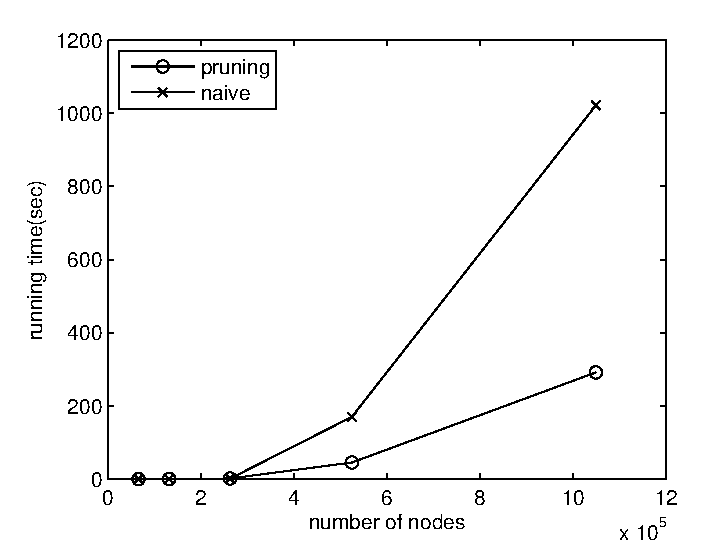
\includegraphics[width=0.7\textwidth]{figs/kronecker}
    \caption{Kronecker graph with 1000 different labels}
    \label{fig:exp:kronecker}
\end{figure}

\begin{table}[h]
    \centering
    \begin{tabular}{|l|l|l|}
    \hline
    datasets                   & Facebook Network & DBLP Network \\ \hline
    number of nodes            & 4039             & 906505       \\ \hline
    number of edges            & 88234            & 1656732      \\ \hline
    number of different labels & 20               & 1000         \\ \hline
    average degree             & 21.8455          & 1.8276       \\ \hline
    \end{tabular}
    \label{tab:exp:fb_dblp}
    \caption{Dataset statistics}
\end{table}

We also do some empirical study on real world datasets. We download a dataset of Facebook network from \emph{Stanford Network Analysis Project} \footnote{\url{http://snap.stanford.edu/data/egonets-Facebook.html}}. In Figure~\ref{fig:exp:fb}, we show the running time of our algorithms in 4-hops neighbourhood with different numbers of unique labels in total. The labels are assigned to the vertices in uniform distribution. In the Facebook network dataset, the running time of the algorithm with pruning is much less than the running time of the algorithm without pruning. We note that neither method is linearly scalable with respect to the size of the graphs. 

\begin{figure}[h]
    \centering
      \includegraphics[width=0.7\textwidth]{figs/FB}
    \caption{Running time of the algorithms on facebook network}
    \label{fig:exp:fb}
\end{figure}

Figure~\ref{fig:exp:fb_dis} shows the distribution of the labels in the Facebook network dataset. The of degrees of most of the vertices are less than 200 while some of the vertices are with degrees greater than 800.

\begin{figure}[H]
    \centering
      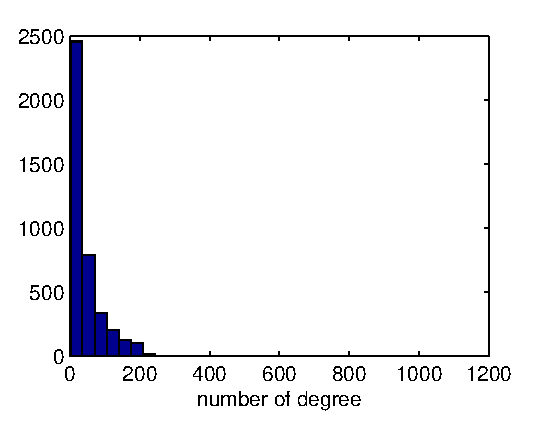
\includegraphics[width=0.5\textwidth]{figs/fb_distri}
    \caption{Facebook network degree distribution}
    \label{fig:exp:fb_dis}
\end{figure}

Figure~\ref{fig:exp:fb_hops} shows the running time of our algorithms with 20 unique labels in different numbers of hops. The speed-up factor of the pruning-based algorithm is increasing with the number of hops.

\begin{figure}[H]
    \centering
      \includegraphics[width=0.5\textwidth]{figs/FB_hops}
    \caption{Running time of the algorithms with different numbers of hops}
    \label{fig:exp:fb_hops}
\end{figure}


We also use the DBLP dataset from $arnetminer$ \footnote{\url{http://arnetminer.org/billboard/citation}} to evaluate the performance of our algorithms. The DBLP dataset provides us the author list of each publication. We build a citation network based on these author lists in the following way. We add an edge between author $X$ and author $Y$ if and only if $X$ is one of the top ten co-authors of $Y$ and $Y$ is one of the top ten co-authors of $X$. We choose the top one thousand most frequent conferences as the labels of the vertices. If an author publishes more than five papers in a conference, then we add the corresponding label of that conference to that vertices. Figure~\ref{fig:exp:dblp} shows that the pruning-based algorithm is about 10 times faster than the algorithm without pruning on DBLP network. We note that neither algorithm is linearly scalable with respect to the size of the graphs.

\begin{figure}[H]
    \centering
      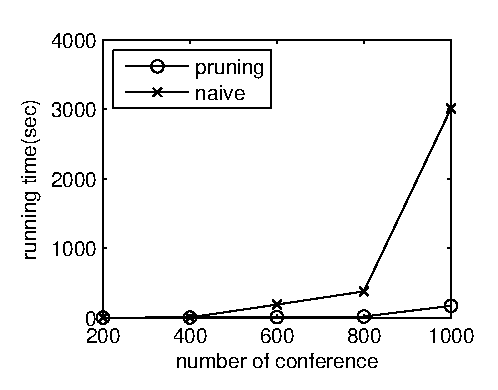
\includegraphics[width=0.7\textwidth]{figs/DBLP}
    \caption{Running time of the algorithms on DBLP network}
    \label{fig:exp:dblp}
\end{figure}

Figure~\ref{fig:exp:dblp_dis} shows the distribution of the degrees of the DBLP network. Comparing to the facebook network, the variance of the degrees of the vertices is not very large.

\begin{figure}[H]
    \centering
      \includegraphics[width=0.5\textwidth]{figs/DBLP_distri}
    \caption{DBLP network degree distribution}
    \label{fig:exp:dblp_dis}
\end{figure}

\section{Experiments of Spatial Skyline Subspace Query}
\label{ch:exp:spatial}
In this section, we will introduce the empirical study on spatial skyline subspace query. We use the Yelp Academic Dataset \footnote{\url{https://www.yelp.ca/academic_dataset}} to evaluate our algorithms. Yelp Academic Dataset provides 13490 different business spots. Each business spot consists of its longitude and latitude information. We use the longitude and latitude information of the business spot as its $XY$ spatial information. The business spot consists of a set of category information, neighbourhood information and university information. We use those information as the labels of the business spot. Each business spot also contains a stars rating.

In Figure~\ref{fig:exp:yelp20l}, we choose the top 20 most popular categories as the labels of the business spot and we compare the running time of the algorithms in the sense of different radii. The running time of the prune-based algorithm is about 2 times faster than the algorithm without pruning.

\begin{figure}[h]
    \centering
      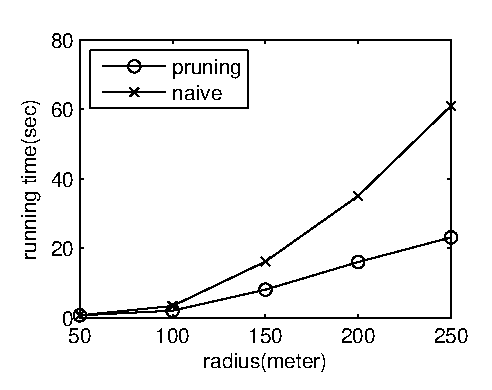
\includegraphics[width=0.7\textwidth]{figs/YelpTop20Labels}
    \caption{Yelp Data Set with Top 20 most popular categories}
    \label{fig:exp:yelp20l}
\end{figure}

In Figure~\ref{fig:exp:yelp300l}, we choose the top $300$ most popular categories as the labels of the business spot. We assign a category to a business spot as a label if the business has the highest star rating among all the business with that category. We note that both algorithms are linearly scalable with respect to radius. Table~\ref{tab:exp:radius} shows the average number of business spots in terms of radius in yelp dataset.

\begin{figure}[h]
    \centering
      \includegraphics[width=0.7\textwidth]{figs/Yelp300Labels}
    \caption{Yelp Data Set with 300 different labels}
    \label{fig:exp:yelp300l}
\end{figure}


\begin{table}[h]
\centering
\begin{tabular}{|l|l|}
\hline
Radius (meters) & Number of Points \\ \hline
50              & 11               \\ \hline
100             & 26               \\ \hline
150             & 42               \\ \hline
200             & 59               \\ \hline
250             & 76               \\ \hline
500             & 159              \\ \hline
1000            & 298              \\ \hline
5000            & 597              \\ \hline
10000           & 657              \\ \hline
20000           & 721              \\ \hline
\end{tabular}
\caption{Number of points in certain radii in average.}
\label{tab:exp:radius}
\end{table}

We also evaluate the running time of the algorithm on data with the radius fixed but the number of labels is different. In this thesis, we conduct the empirical study on the large neighbourhood queries whose label collection radius is 10000 meters. we first get a random permutation of the labels. Second, we run our programs on the first $100$ labels, the first $200$ labels, $\dots$, etc. Figure~\ref{fig:exp:yelp10k} shows the running time per query in average. The running time of the pruning-based algorithm does not have significant better performance than the algorithm without pruning.

\begin{figure}[h]
    \centering
      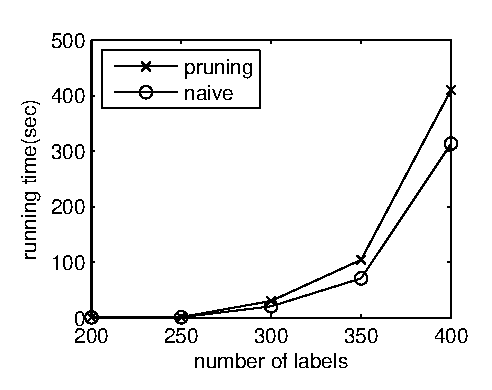
\includegraphics[width=0.7\textwidth]{figs/Yelp10Kmeters}
    \caption{Yelp Data Set in 10000 meters neighbourhood}
    \label{fig:exp:yelp10k}
\end{figure}

Figure~\ref{fig:exp:spatial} shows the running time of spatial synthetic data with 20 different labels. Both the spatial points and the labels of the points are generated randomly in uniform distribution. The pruning-based algorithm is 7 times faster than the naive algorithm when the radius is 40000.

\begin{figure}[h]
    \centering
        \includegraphics[width=0.7\textwidth]{figs/Spatial}
    \caption{Spatial Synthetic Dataset}
    \label{fig:exp:spatial}
\end{figure}

In summary, the experimental result shows that our algorithms compute the skyline subspace efficiently and the pruning methods improve the running time of the programs effectively.
%% Copyright 1998 Pepe Kubon
%%
%% `two.tex' --- 2nd chapter for thes-full.tex, thes-short-tex from
%%               the `csthesis' bundle
%%
%% You are allowed to distribute this file together with all files
%% mentioned in READ.ME.
%%
%% You are not allowed to modify its contents.
%%

%%%%%%%%%%%%%%%%%%%%%%%%%%%%%%%%%%%%%%%%%%%%%%%%%
%
%     Chapter 7  
%
%%%%%%%%%%%%%%%%%%%%%%%%%%%%%%%%%%%%%%%%%%%%%%%%

\chapter{Conclusions}
\label{ch:con}
%\section{Summary of the Thesis}

The skyline subspace problem is originally motivated by the problem of what distinguish one from its peers in social networks~\cite{lo2013distinguish}. In this thesis, we formulate the social network into a graph with labels and consider the distances between a person and the labels as the factors that distinguish the person from its peers. We propose an bottom-up algorithm to answer \emph{skyline subspace query} which is based on set enumeration and dominating candidate sets intersection. To tackle the problems of skyline subspaces on graph and the skyline subspaces on euclidean space, we develop effective pruning methods to reduce the search space. 
We did empirical studies using both synthetic and real data sets to evaluate our approach. We generated the synthetic graph based on the Kronecker graph model and the real world datasets are from DBLP and YELP. The experimental results verify the efficiency of our algorithms.

%\section{Future Work}
% Our methods can be improved in several aspects. In general, we can take advantage of pruning techniques used in static similarity join and search algorithms. We may also want to generalize the signature-based method for more similarity measures. 

As for future work, we can consider the following directions.  

\begin{itemize}
% \item We can take advantage of pruning techniques used in static similarity join and search algorithms.
% \item We may also want to generalize the signature-based method for more similarity measures. For example, Random projection method of LSH.      
   
\item \textit{Using top-down set enumeration.} Our algorithm is based on bottom-up set enumeration. In bottom-up manner, We take the advantage of the property that if a target skyline subspace is found then we do not need to search for the subspaces that contain this subspace. For top-down approach, one of the advantage we can take is that if the query point is strictly dominated by some points in a certain subspace $\mathcal{A}$, then we do not need to check the subsets of the subspace $\mathcal{A}$ because we know that the query point can not be a skyline point in those subspaces.

\item \textit{Further pruning method development in euclidean space} There are many properties in euclidean space. In~\cite{sharifzadeh2006spatial}, Sharifzadeh et al. took the advantage of property of convex hull to reduce the size of skyline candidates. They also used the Voronoi diagram structure to index the graph. For future work, we can index the spatial points using Voronoi diagram instead of R-tree and applied pruning methods based on some geometry properties such as the property of convex hull.

\item \textit{Voronoi Diagram}     


\end{itemize}

















%%%%%%  bibliography
%\include{files/bibl}
\addcontentsline{toc}{chapter}{Bibliography}
\typeout{Bibliography}
\bibliographystyle{abbrv}
\bibliography{topk}
\renewcommand{\baselinestretch}{\textstretch} %% get normal spacing
\normalsize


%%%  appendices, if any
%\begin{appendices}
%\include{files/appone}
%\include{files/apptwo}
%\end{appendices}


%%%%%%  index
\include{files/ind}

\end{document}







%%% Local Variables: 
%%% mode: latex
%%% TeX-master: t
%%% End: 
